\chapter{Introduction}\label{chap:1}
Technology and the impact it is having in our society is changing the way we think and the way we interact with each other. With more and more automation in the workplace many monotonous jobs are disappearing and more creative ones are replacing them. This and the fact that technology has opened the mind and ability for people to start a business as the cost to startup a business thanks to technology has greatly reduced.
The objective of this project is to automate the personal training area as it has been relatively untouched. The problem is that many people unknowingly train in a way that in the long term may cause them injury, this is due to the lack of knowledge and guidance to train differently and safely. Gym trainers may provide some guidance but with the amount of people normally in these gyms they can’t be always there to help. The idea is to create a chatbot that can aid, track progress and create training sessions that adapt to each user whenever the user needs them. 
\section{Background}\label{sec:chap1_background}
Machine Learning (ML) algorithms in recent years have improved greatly thanks to the immense computing power available. This with the amount of data currently accessible, has naturally led the way for the development of bots that can communicate with people, originally with basic phrases and over time in a more complex and natural manner. New technologies have made it more intuitive and easier to work on this area with many Natural Language Processing (NLP) libraries such as Natural Language Tool Kit (NLTK) that help translate human spoken phrases to something easier for the computer to understand. Other libraries like TensorFlow or Scikit-Learn provide functionality to train models based on the processing done in NLTK.
Nowadays, even though the libraries mentioned before are still frequently used, it is more common now to see platforms that abstracts the users from the inner workings of the algorithms and instead leaves the user with an intuitive UI for the user to create their own functionality for the chatbot.

Thanks to the access we have now to smartphones and social platforms the integration of chatbots in these platforms is growing steadily as it allows the user to communicate with help centers without waiting a long time to get a response.

\section{Motivation}\label{sec:chap1_moti}
The motivation to develop this project comes from the time-consuming activity of preparing a time table with what muscles and exercises to train and the forgetful way of tracking a person’s progress when going to the gym, for this reason, with the knowledge acquired over the years and the technology available this project came to life. It is not only a project to finish the degree it is a project that after giving it in will still be worked on over time to add more functionality and make it a truly useful application that can be used by users outside the University environment. This will be more of a proof of concept to verify the viability of further developing and investing the time to add more functionality.

\section{Development Stages}\label{sec:chap1_dev-stag}
The project has gone though several makeovers due to the time constraint to develop the chatbot. 
\subsection{Planification}\label{sec:chap1_plan}
Originally the idea was to use a structure like a project done previously where a virtual machine in Google Cloud was the brains of the bot. In this project as there was access to a raspberry pi, the idea to use a cloud provider was changed to have it be the server. 
In this stage, the most time was spent on how the architecture of the bot was going to be and what technologies was going to be used throughout the project. This planning has had to be revised several times changing the whole architecture from a proprietary solution using several of the libraries mentioned before in the background to an open source platform called Rasa. Also, due to continuous problems caused by the raspberry pi with the installation of libraries and the lack of computing power the decision was to change the server to Azure, Microsof’s Cloud Service.
\subsection{Development}\label{sec:chap1_dev}
In this stage is where all the planning came to life and where most of the time was spent. It was composed of two plans. \\\\
\textbf{Inicial plan:}
\begin{itemize}
	\item{\textbf{Creation of a webhook to manage incoming messages from telegram in the server.}}
	\item{\textbf{DB creation to manage user info.}}
	\item{\textbf{User recognition.}}
	\item{\textbf{Intent Detection using NLTK and Scikit-learn.}}
	\item{\textbf{Conversation flows (unfinished due to complexity and time constraint).}}
\end{itemize}
\textbf{Revised plan:} \\\\
	Due to the time to create a context manager for complex conversational flows and the limit imposed by time, half way through the development it was decided to redo everything with Rasa.
\begin{itemize}
	\item{\textbf{Reconfigure webhook to manage incoming messages with rasa.}}
	\item{\textbf{Conversation stories creation.}}
	\item{\textbf{Entity extraction.}}
\end{itemize}

\section{Resources Used}\label{sec:chap1_res}
As it was said in the previous point there were two different plans, for the original one the resources used were:\\	
\begin{itemize}
	\item{\textbf{Telegram:} This was used as the platform for the user to communicate with the bot as it supports it, there are other platforms that can be used as well as integrating them isn’t complicated, but as a proof of concept telegram works well.}
	\item{\textbf{Raspberry pi:} Used as the server to hold the brains of the chatbot. Limited in computing power.}
	\item{\textbf{Python:} The programming language by excellence for machine learning as it is intuitive and has a lot of community support. The main libraries used for this original plan were:
		\begin{itemize}
			\item{\textbf{NLTK:} For the translation from human language to something the computer understands.}
			\item{\textbf{Scikit-learn:} For training and classifying the models for the bot.}
			\item{\textbf{Pickle:} To store the bot’s trained models.}
			\item{\textbf{CSV:} To load the training data from a csv file.}
		\end{itemize}	 
	}
\end{itemize}
For the revised plan a few things changed:
\begin{itemize}
\item{The raspberry pi was changed to a cloud solution by Microsoft called Azure, this virtual machine has double the ram of the raspberry pi and a higher computing power making the bot train quicker.}
\item{Even though Python is still used in this revised plan, the libraries are packaged in to the new Natural Language Engine, Rasa which takes care of training the bot.}
\end{itemize}
	
\section{Memory Structure}\label{sec:chap1_mem-str}
The document is structured in different sections where the different aspects of the project will be explained.
\begin{itemize}
	\item{\textbf{Analysis of the problem:} An in-depth analysis off the current state of the gym sector and why the need for a personal assistant is required for improving the overall efficiency when a user is working out. In this section the objectives of what this project is trying to achieve will be explained.}
	\item{\textbf{State of the art:} An analysis on how the ML and NLP technologies have evolved to the current state and where it is currently heading. What rol are chatbots taking in society.}
	\item{\textbf{Solution proposed:} How the solution provided in this project can benefit millions of people and how this project has been developed as well as the regulatory framework surrounding virtual assistants and user data manipulation.}
	\item{\textbf{Planning and budget:} How the original planning was made and how it compares to the real development. Also, this section reviews how much budget this project has taken.}
	\item{\textbf{Socioeconomic Environment:} An approach on how the current chatbot technology is changing many industries and saving costs for companies and providing a better service for their clients.}
\end{itemize}
%\begin{center}
%\begin{figure}[h!]
% \centering
%   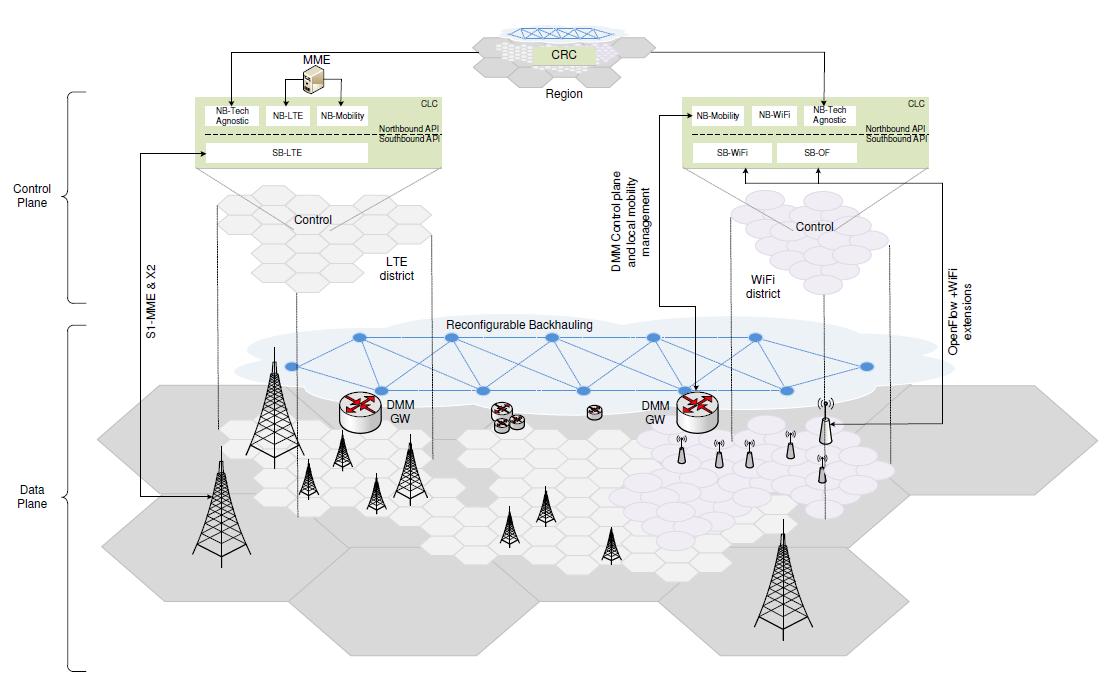
\includegraphics[scale=0.5]{./images/crowd_arch}
%	\caption{CROWD Architecture}
%	\label{crowd_arch-fig}
%\end{figure}
%\end{center}















